\documentclass[17pt,landscape]{foils}
\usepackage[latin1]{inputenc}
\usepackage[T1]{fontenc}
\usepackage[french]{babel}
\usepackage{amsmath,amsthm}
\usepackage{amssymb}
\usepackage{fancyhdr}
\usepackage[pdftex]{graphicx,graphics,color}
\usepackage[colorlinks]{hyperref}
\cfoot{\small{}} \pagestyle{fancy} \hypersetup{pdftitle={A mixed
linear model with change-points for the analysis multiple patients
of CGH data},
           pdfauthor={Emilie LEBARBIER},
           pdfpagemode={FullScreen}
}


\textwidth 24cm \textheight 20cm \topmargin 0cm \oddsidemargin 0cm
\evensidemargin 0cm

\newcommand{\coefbin}[2]{\left(
    \begin{array}{c} #1 \\ #2 \end{array}
  \right)}
  \newcommand{\Bcal}{\mathcal{B}}
\newcommand{\Ccal}{\mathcal{C}}
\newcommand{\Dcal}{\mathcal{D}}
\newcommand{\Ecal}{\mathcal{E}}
\newcommand{\Gcal}{\mathcal{G}}
\newcommand{\Mcal}{\mathcal{M}}
\newcommand{\Ncal}{\mathcal{N}}
\newcommand{\Pcal}{\mathcal{P}}
\newcommand{\Qcal}{\mathcal{Q}}
\newcommand{\Lcal}{\mathcal{L}}
\newcommand{\Tcal}{\mathcal{T}}
\newcommand{\Ucal}{\mathcal{U}}
\newcommand{\alphabf}{\mbox{\mathversion{bold}{$\alpha$}}}
\newcommand{\betabf}{\mbox{\mathversion{bold}{$\beta$}}}
\newcommand{\gammabf}{\mbox{\mathversion{bold}{$\gamma$}}}
\newcommand{\mubf}{\mbox{\mathversion{bold}{$\mu$}}}
\newcommand{\thetabf}{\mbox{\mathversion{bold}{$\theta$}}}
\newcommand{\Pibf}{\mbox{\mathversion{bold}{$\Pi$}}}
\newcommand{\psibf}{\mbox{\mathversion{bold}{$\psi$}}}
\newcommand{\Sigmabf}{\mbox{\mathversion{bold}{$\Sigma$}}}
\newcommand{\taubf}{\mbox{\mathversion{bold}{$\tau$}}}
\newcommand{\Ebf}{{\bf E}}
\newcommand{\Gbf}{{\bf G}}
\newcommand{\Hbf}{{\bf H}}
\newcommand{\Ibf}{{\bf I}}
\newcommand{\mbf}{{\bf m}}
\newcommand{\Obf}{{\bf 0}}
\newcommand{\Rbf}{{\bf R}}
\newcommand{\Sbf}{{\bf S}}
\newcommand{\Tbf}{{\bf T}}
\newcommand{\Ubf}{{\bf U}}
\newcommand{\Vbf}{{\bf V}}
\newcommand{\xbf}{{\bf x}}
\newcommand{\Xbf}{{\bf X}}
\newcommand{\Ybf}{{\bf Y}}
\newcommand{\Zbf}{{\bf Z}}
\newcommand{\Esp}{{\mathbb E}}
\newcommand{\Var}{{\mathbb V}}
\newcommand{\Cov}{{\mathbb C}\mbox{ov}}
\newcommand{\Ibb}{{\mathbb I}}
\newcommand{\Rbb}{\mathbb{R}}
\renewcommand{\baselinestretch}{1.3}
\newdimen\AAdi%
\newbox\AAbo%
\newcommand{\emphase}[1]{\textblue{\sl #1}}
\def\argmax{\mathop{\mathrm{argmax}}}

\title{\large{A mixed linear model with breakpoints for the
analysis of multiple CGH arrays}}

\author{ E. Lebarbier, S. Robin \\
      \footnotesize {UMR INA P-G/ENGREF/INRA MIA 518, Paris, France} \\
      F. Picard \\
      \footnotesize {UMR CNRS-8071/INRA-1152/Universit\'e d'\'Evry, \'Evry, France}\\
      Eva Budinsk\`a \\
      \footnotesize {Centre of Biostatistics and Analyses, Faculty of Science and Faculty
of Medicine, Masaryk University, Brno}  \\ \\ \\
  %\hspace{-3cm}
   {SMAI June 4-8, 2007}  }



\date{}

\begin{document}


\maketitle \MyLogo{}
\definecolor{gris}{rgb}{0.9,0.9,0.9}
\definecolor{bleufonce}{rgb}{0,0,0.5}
%\color{bleufonce} %\pagecolor{gris}
\newcommand{\textblue}[1]{\textcolor{blue}{#1}}
\newcommand{\section}[1]{\centerline{\large \textblue{#1}}}
\newcommand{\paragraph}[1]{\noindent {\textblue{#1}}}
\newcommand{\textred}[1]{\textcolor{red}{#1}}
\newcommand{\textgreen}[1]{\textcolor{green}{ #1}}
%%%%%%%%%%%%%%%%%%%%%%%%%%%%%%%%%%%%%%%%%%%%%%%%%%%%%%%%%%%%%%%%%%%%%%%%%%%%%%%%%%%%%%%%%
%--------------------------------- CGH technology --------------------------------
%%%%%%%%%%%%%%%%%%%%%%%%%%%%%%%%%%%%%%%%%%%%%%%%%%%%%%%%%%%%%%%%%%%%%%%%%%%%%%%%%%%%%%%%
\newpage
\chead{\large {CGH microarray technology}} \foilhead[-.5in]{}

%\vspace{-0.3cm}

\paragraph{Objective.} Detection of chromosomal aberrations (within chromosome).

\paragraph{CGH = Comparative Genomic Hybridization.} Method for the
  comparative measurement of relative DNA copy numbers between two
  samples (normal/disease, test/reference).
\centerline{$\rightarrow$ Application of the \textblue{microarray}
    technology to CGH (resolution $\sim$ 100kb).}


\paragraph{Microarray technology in its principle.}

\vspace{-0.5cm}


\begin{figure}
\begin{center}
\includegraphics[scale=0.47]{principe_CGH.png}
\end{center}
\end{figure}

%%%%%%%%%%%%%%%%%%%%%%%%%%%%%%%%%%%%%%%%%%%%%%%%%%%%%%%%%%%%%%%%%%%%%%%%%%%%%%%%%%%%%%%%%
%--------------------------------- CGH profile --------------------------------
%%%%%%%%%%%%%%%%%%%%%%%%%%%%%%%%%%%%%%%%%%%%%%%%%%%%%%%%%%%%%%%%%%%%%%%%%%%%%%%%%%%%%%%%
\newpage
\chead{\large {Interpretation of a CGH profile}} \foilhead[-.5in]{}



\begin{figure}
\begin{center}
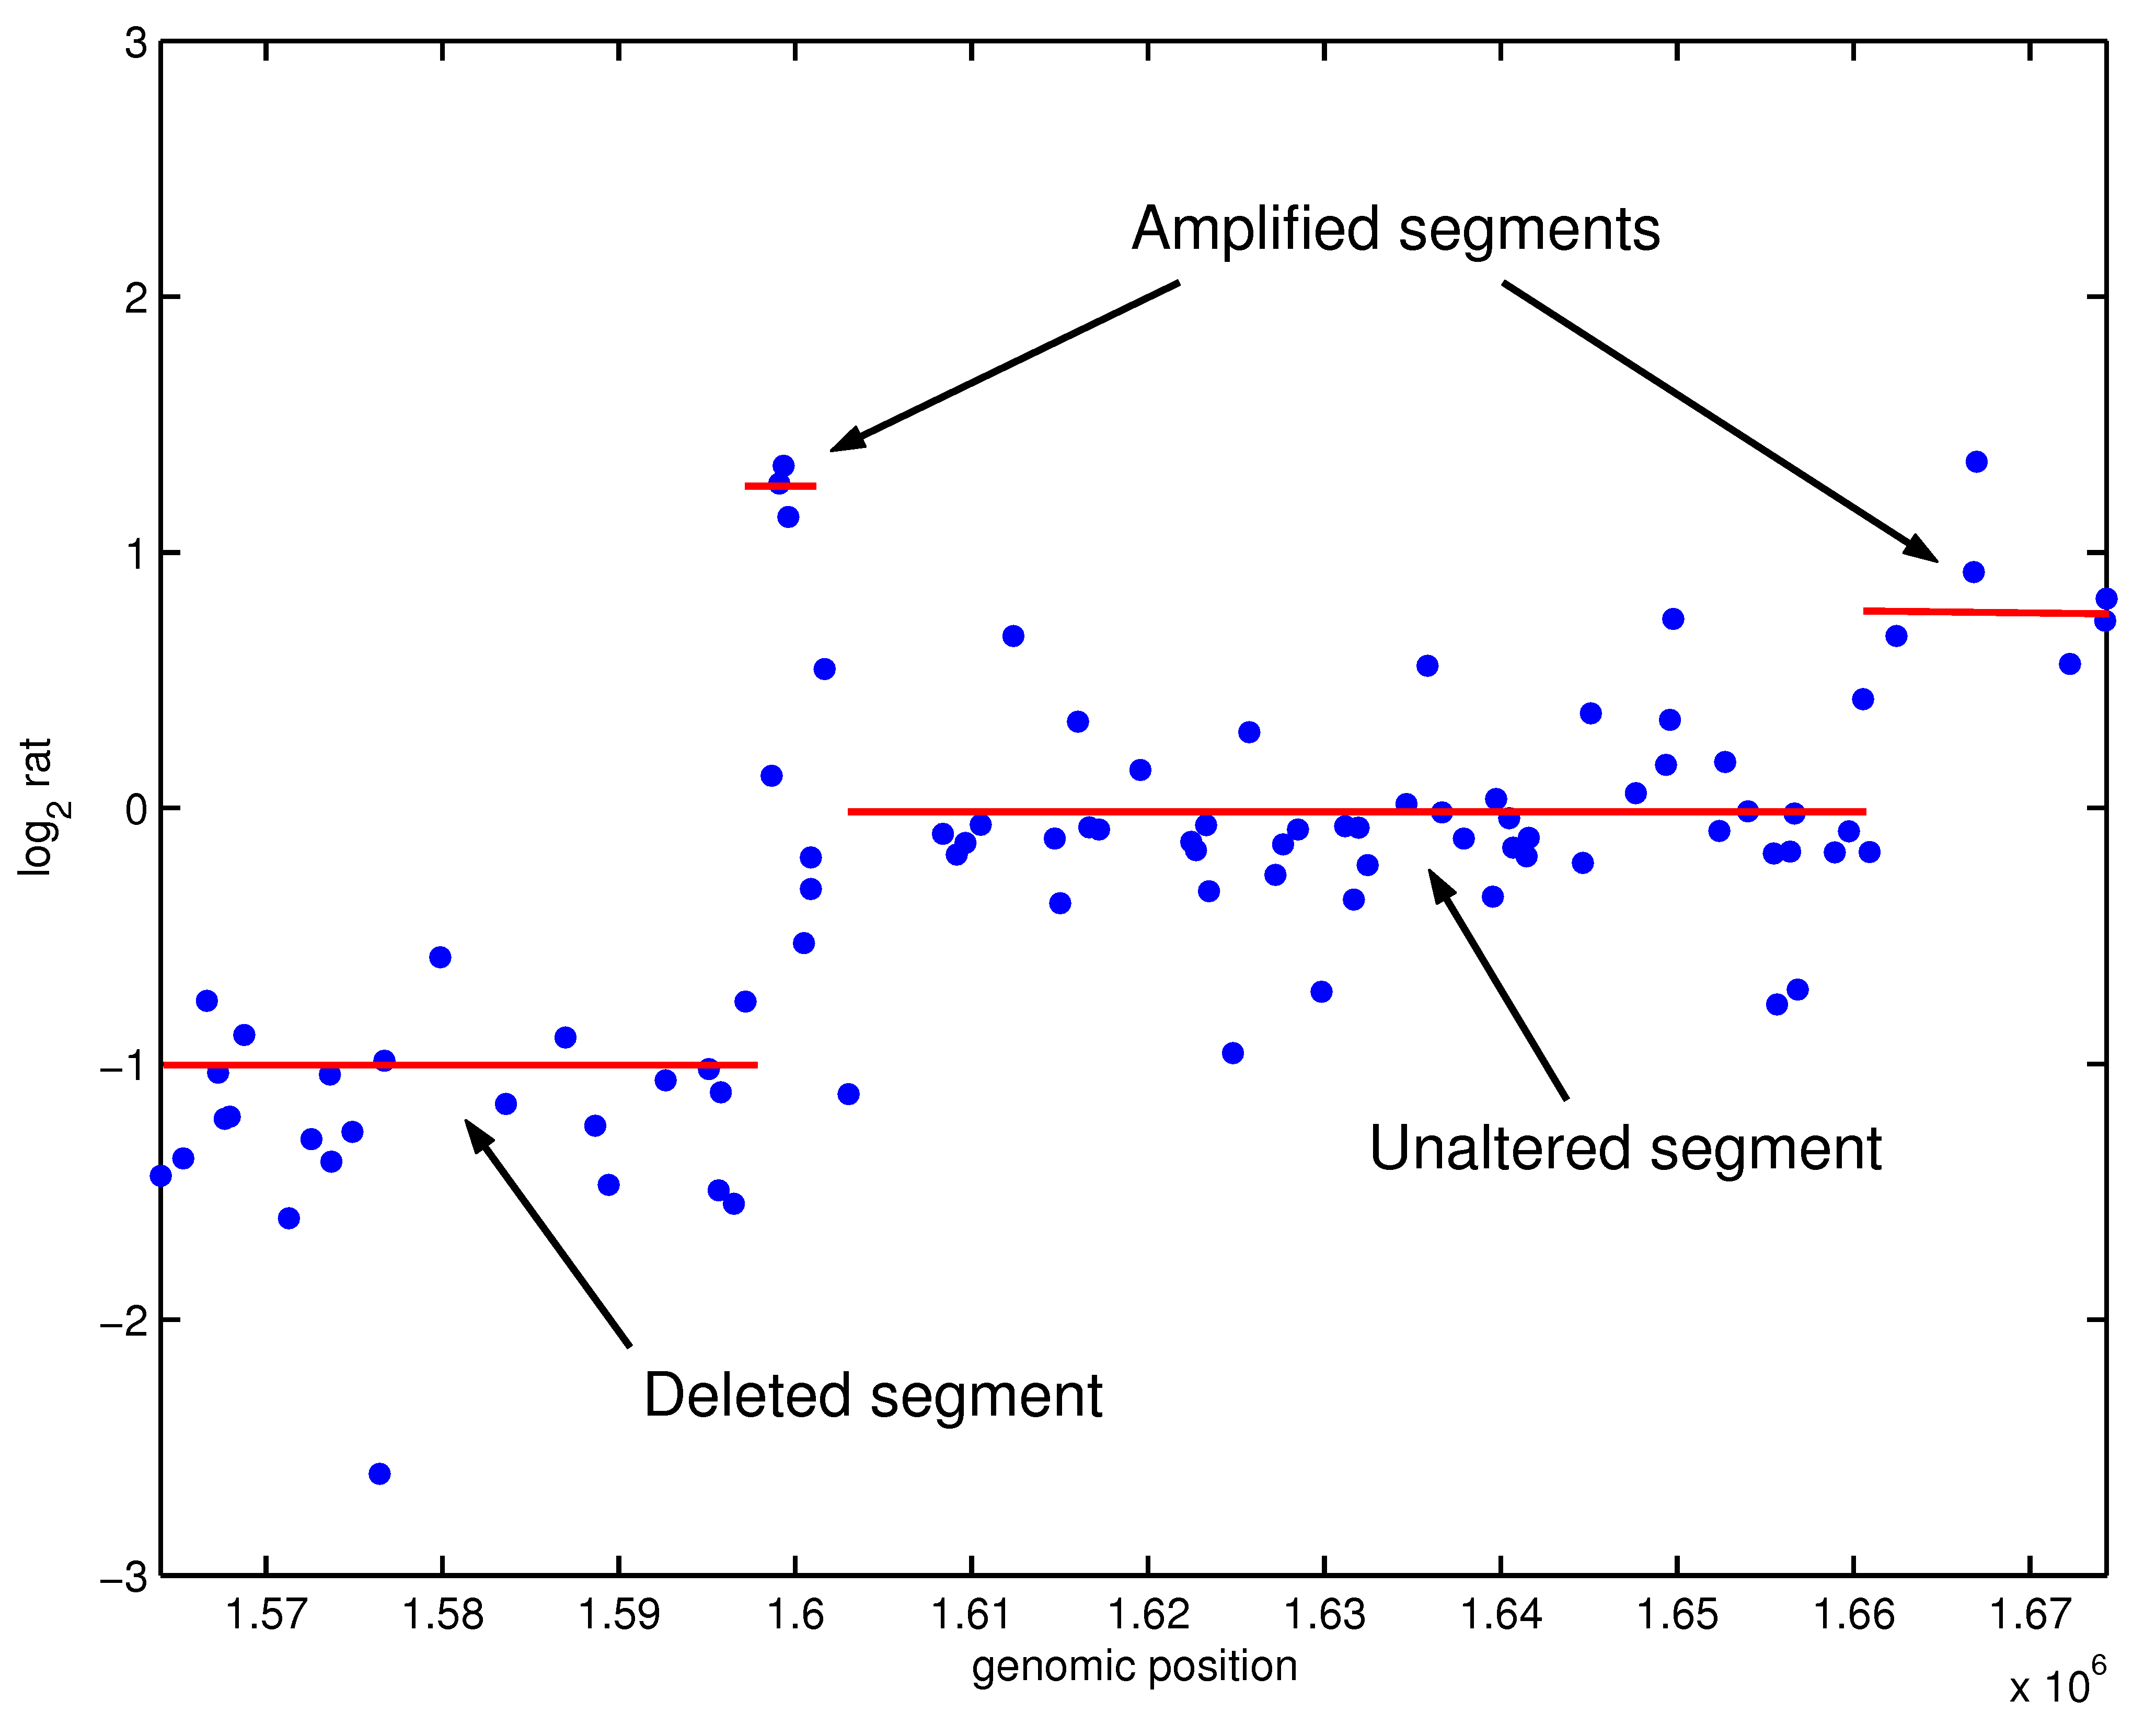
\includegraphics[scale=0.8]{profile_example.png}
\end{center}
\end{figure}

\vspace{0.2cm}

\centerline{
  A dot on the graph
  $
  \displaystyle{
    = \log_2 \left\{ \frac{\text{ $\sharp$ copies of BAC(t) in the test
          genome }}{\text{$\sharp$ copies of BAC(t) in the reference
          genome}}\right\}}
  $
}


%%%%%%%%%%%%%%%%%%%%%%%%%%%%%%%%%%%%%%%%%%%%%%%%%%%%%%%%%%%%%%%%%%%%%%%%%%%%%%%%%%%%%%%%%
%--------------------------------- Mod�le de d�tection de ruptures --------------------------------
%%%%%%%%%%%%%%%%%%%%%%%%%%%%%%%%%%%%%%%%%%%%%%%%%%%%%%%%%%%%%%%%%%%%%%%%%%%%%%%%%%%%%%%%
\newpage
\chead{\large {Breakpoint detection Model \small{(Work of Picard et
al. (2005))}}} \foilhead[-.5in]{}



\paragraph{Model.} The observed signal $Y=(Y_1,\ldots,Y_n)$ is such that :
$$
Y_t=\mu_k + E_t \ \ \ \  \mbox{ if position $t$ is in segment
$I_k=[t_{k-1}+1,t_{k}]$,}
$$
with $\{E_t\}$ i.i.d. $\sim \Ncal(0,\sigma^2)$ and $k=1,\ldots,K$.

%\vspace{-.2cm}

\paragraph{The parameters of this model are} $T  =  (t_1, ..., t_{K-1})$ and $\Theta  =
(\mu_1,\hdots,\mu_K,\sigma^2)$.


\paragraph{Parameter estimation by maximum likelihood}

$\rightarrow$ To find the breakpoints, we have to minimize
$\sum_{k=1}^K \sum_{t \in I_k} (Y_t - \widehat{\mu}_k)^2.$

$\rightarrow$ impossible to explore all possible segmentations for
large $n$ and $K$.

$\rightarrow$ Solution: \emphase{dynamic programming} can be used
since the contrast to be minimized is additive in $K$.

\paragraph{Choice of $K$.} Model selection: Penalized
Log-Likelihood.





%%%%%%%%%%%%%%%%%%%%%%%%%%%%%%%%%%%%%%%%%%%%%%%%%%%%%%%%%%
%%%%%%%%%%%%%%%%%%%%%%%%%%%%%%%%%%%%%%%%%%%%%%%%%%%%%%%%%%
\newpage
\chead{\large {Multiple arrays analysis}} \foilhead[-.5in]{}

\vspace{1cm}

\paragraph{Example : comparing groups of patients}
To detect chromosomal aberrations associated with a specific
disease, we compare the profiles of healthy and disease patients, or
the profiles of group of patients with different prognosis.


\paragraph{Common breakpoints:} all patients within the same group have their breakpoints at the
same positions.\\
 This can be done with a generalization of the
model presented above but this is not relevant biologically.

\paragraph{Proposed model.}

$\rightarrow$ We allow patient-specific segmentation.

$\rightarrow$ \emphase{Assumption:} the profiles of patients within
a same group at same position are \emphase{correlated}.



%%%%%%%%%%%%%%%%%%%%%%%%%%%%%%%%%%%%%%%%%%%%%%%%%%%%%%%%%%
\newpage
\chead{\large {Mixed linear model with breakpoints}}
\foilhead[-.5in]{}

\vspace{-0.5cm}

\paragraph{Model.} $Y_{g\ell t}$ denotes the observed logratio at position $t$
for patient $\ell$ within group $g$. We assume that
$$
Y_{g\ell t} = \mu_{g\ell k} + U_{gt} + E_{g\ell t} \qquad \mbox{if
position $t$ belongs to segment $I_{g\ell k}$}
$$
where
\begin{itemize}
\item $I_{g\ell k}$ is the $k$-th segment of patient
  $\ell$ from group $g$,
\item  $\mu_{g\ell k}$ is the mean signal in segment
  $I_{g\ell k}$,
\item  $U_{gt}$ is the random effect at position $t$ in
  group $g$: $\{U_{gt}\}$ independent, $U_{gt} \sim \Ncal(0,
  \sigma^2_g)$,
\item $E_{g\ell t}$ is the noise: $\{E_{g\ell t}\}$
  i.i.d. $\sim \Ncal(0, \sigma^2_0)$.
\end{itemize}

\vspace{-.5cm}

$$
\Cov(Y_{g\ell t}, Y_{g'\ell' t'}) =  \sigma^2_g \quad \mbox{ if
  \textblue{same group $g$ and same position $t$}}.
$$


\paragraph{General model}
$$
\Ybf = \underset{\mbox{Covariates}}{\underbrace{\Xbf \thetabf}} +
\underset{\mbox{Segmentation}}{\underbrace{\Tbf \mubf}} +
\underset{\mbox{Random effect}}{\underbrace{\Zbf \Ubf}} + \Ebf
$$
with $\Ebf \sim \Ncal(\Obf, \Rbf)$, \emphase{$\Rbf$ diagonal}






%%%%%%%%%%%%%%%%%%%%%%%%%%%%%%%%%%%%%%%%%%%%%%%%%%%%%%%%%%
\newpage
\chead{\large {Parameters estimation}} \foilhead[-.5in]{}



\paragraph{Direct maximisation of the likelihood.}
The distribution of $\Ybf$ is
$$
\Ybf \sim \Ncal(\Xbf \thetabf + \Tbf \mubf, \Vbf), \qquad
\mbox{where
  } \Vbf = \Zbf \Gbf \Zbf' + \Rbf.
$$
Because, $\Vbf$ is not diagonal, the direct maximisation of the
observed log-likelihood $\Lcal(\Ybf)$ leads to the minimisation of a
non additive contrast in $K$.

\centerline{Dynamic programming \emphase{can not be used} to
estimate
  $\Tbf$ and $\mubf$}




\paragraph{Idea.}
$$
\Ybf -\Xbf \thetabf - \Zbf \Ubf \; | \; \Ubf \sim \Ncal(\Tbf \mubf,
\Rbf).
$$
$\Rbf$ is diagonal so the contrast to be minimized is additive in
$K$.

\centerline{\emphase{Dynamic programming can be used to estimate
    $\Tbf$ and $\mubf$}}

\paragraph{E-M strategy.} (used by Foulley (Lecture note, 2004) for mixed linear models) the
unobserved effect $\Ubf$ is predicted.




%%%%%%%%%%%%%%%%%%%%%%%%%%%%%%%%%%%%%%%%%%%%%%%%%%%%%%%%%%
\newpage
\chead{\large {E-M algorithm}} \foilhead[-.5in]{}

\paragraph{Idea.} The model can be viewed as model with incomplete data
: \emphase{$U$ is hidden}.


\paragraph{Principle.}
In presence of incomplete data, the maximisation of $\Lcal(\Ybf)$ is
equivalent to the maximisation of the conditional expectation
$$
\Qcal = \Esp\left[\Lcal(\Ybf, \Ubf) \; | \; \Ybf \right] =
\underset{\mbox{$\Qcal_0$}}{\underbrace{\Esp\left[\Lcal(\Ybf| \Ubf)
\; | \; \Ybf \right]}} +
\underset{\mbox{$\Qcal_1$}}{\underbrace{\Esp\left[\Lcal(\Ubf) \; |
\; \Ybf \right]}}.
$$

Here we have
\begin{eqnarray*}
  -2\Qcal_0 & = & N\log(2 \pi \sigma^2_0) + \left [ \mbox{\rm Tr}\left[ \Zbf
  \Var(\Ubf|\Ybf) \Zbf'\right] + \|\Ybf - \Xbf\thetabf -
    \Tbf\mubf - \Zbf\Esp(\Ubf|\Ybf) \|^2  \right ] /\sigma^2_0 \\
  \\
  -2\Qcal_1 & = & \sum_g \left[M \log(2\pi\sigma^2_g) +
  \Esp(\Ubf_g'\Ubf_g | \Ybf)/\sigma^2_g \right].
\end{eqnarray*}


%& = & -\frac{1}{2} \left [ M \log(2\pi)+ \log(|\Gbf|)\right ]\\
%              &&-\frac{1}{2} M \text{Tr} \left(\Gbf^{-1}\left[ \ec{\Ubf} \ec{\Ubf}'+\vc{\Ubf} \right] \right)

%%%%%%%%%%%%%%%%%%%%%%%%%%%%%%%%%%%%%%%%%%%%%%%%%%%%%%%%%%
\newpage
\chead{\large {E-M algorithm }} \foilhead[-.5in]{}

\paragraph{E-step.} To calculate $\Qcal$, we need the following estimates
\begin{eqnarray*}
  \widehat{\Esp}(\Ubf|\Ybf) & = & \Gbf \Zbf' \Vbf^{-1} (\Ybf - \Xbf\thetabf -
  \Tbf\mubf)\\
  \widehat{\Var}(\Ubf|\Ybf) & = & \Gbf - \Gbf \Zbf' \Vbf^{-1} \Zbf
  \Gbf
\end{eqnarray*}

\vspace{-1cm}

where $\Vbf^{-1}$ is calculated using Henderson's trick.

\paragraph{M-step.} Denoting $\widehat{\Ubf} =
\widehat{\Esp}(\Ubf|\Ybf)$ , we get parameter estimates as follows:
\begin{eqnarray*}
\widehat{\sigma}^2_g & = & \arg\max_{\sigma^2_g} \Qcal_1, \\
\widehat{\sigma}^2_0 & = & \arg\max_{\sigma^2_0} \Qcal_0, \\
\widehat{\thetabf} & = & (\Xbf'\Xbf)^{-1} \Xbf'(\Ybf - \widehat{\Tbf
\mubf}
    -\Zbf \widehat{\Ubf}), \\
\widehat{\Tbf \mubf} & = & \arg\min_{\Tbf\mubf} \|\Ybf -
\Xbf\widehat{\thetabf}-{\Tbf\mubf}-\Zbf \widehat{\Ubf})\|^2.
\end{eqnarray*}

\vspace{-1cm}

The last maximisation (segmentation) is achieved thanks to dynamic
programming.


%%%%%%%%%%%%%%%%%%%%%%%%%%%%%%%%%%%%%%%%%%%%%%%%%%%%%%%%%%
%%%%%%%%%%%%%%%%%%%%%%%%%%%%%%%%%%%%%%%%%%%%%%%%%%%%%%%%%%
\newpage
\chead{\large {Implementation strategies}} \foilhead[-.5in]{}


\paragraph{Segmentation step.} The  step is computationally
heavy. We use a two stage dynamic programming algorithm. \\

\paragraph{'Regular' EM.} During the M step, $\Qcal$ is supposed to
be maximised. The circular estimation of $\sigma^2_g, \sigma^2_0,
\thetabf$ and $\Tbf\mubf$ given $\widehat{\Ubf}$ and
$\widehat{\Var}(\Ubf|\Ybf)$ until convergence could achieve this
task, but it would requires \emphase{numerous dynamic programming
steps}
at each M step.\\

\paragraph{Proposed strategy.} To perform few dynamic programming
steps, we iterate the E step and the circular estimation of
$\sigma^2_g, \sigma^2_0$ and $\thetabf$ until convergence, before
updating $\widehat{\Tbf\mubf}$.\\
$\rightarrow$ this is a type of GEM strategy : $Q$ increases at each
step.\\

\paragraph{Numerical comparison.} The two algorithms give the
\emphase{same estimates}, but the proposed strategy is the
\emphase{most efficient} in terms of computational time.


%%%%%%%%%%%%%%%%%%%%%%%%%%%%%%%%%%%%%%%%%%%%%%%%%%%%%%%%%%
\newpage
\chead{\large {Selection of the number of segments $K$}}
\foilhead[-.5in]{}

\paragraph{The total number of breakpoints $K$} is unknown.

\paragraph{Model selection.}
\begin{equation*}
\widehat{K}=\argmax_{K} \left \{ \Lcal(\Ybf; \widehat{\phi})-pen(K)
\right \}
\end{equation*}

\paragraph{Penalty.}

\begin{equation*}
pen(K)=\alpha \left \{ \text{Number of parameters of model of
K-dimensional} \right \} \left( 2 \log{N/K}+5 \right )
\end{equation*}


\paragraph{Calibration of $\alpha$} by adaptative method (Birg� and Massart (2004)).

%%%%%%%%%%%%%%%%%%%%%%%%%%%%%%%%%%%%%%%%%%%%%%%%%%%%%%%%%%
%%%%%%%%%%%%%%%%%%%%%%%%%%%%%%%%%%%%%%%%%%%%%%%%%%%%%%%%%%
\newpage
\chead{\large {Application on Nakao dataset (Nakao et al (2004))-
chromosome 20}} \foilhead[-.5in]{}

\vspace{0.2cm}


\begin{center}
\begin{tabular}{ccc}
  & Stage 1 (11 patients) & Stage 2 (37 patients) \\
  \hspace{-1cm}
  & \begin{tabular}{c}
  \includegraphics[scale=0.45]{hist_ruptures_nakao20_group_Kh=360_group1.png}
  \end{tabular}  &
  \begin{tabular}{c}
  \includegraphics[scale=0.45]{hist_ruptures_nakao20_group_Kh=360_group2.png}
  \end{tabular} \\
 \begin{tabular}{p{5.5cm}} \emphase{Number of breakpoints} \end{tabular} & \\
 \begin{tabular}{p{3.5cm}} \emphase{($\hat{K}$=240)} \end{tabular}&  Stage 3 (35 patients) & Stage 4 (38 patients) \\
  \hspace{-1cm}
 & \begin{tabular}{c}
  \includegraphics[scale=0.45]{hist_ruptures_nakao20_group_Kh=360_group3.png}
  \end{tabular}  &
  \begin{tabular}{c}
  \includegraphics[scale=0.45]{hist_ruptures_nakao20_group_Kh=360_group4.png}
  \end{tabular}
\end{tabular}
\end{center}

%%%%%%%%%%%%%%%%%%%%%%%%%%%%%%%%%%%%%%%%%%%%%%%%%%%%%%%%%%
\newpage
\chead{\large {What is the role of the random effect?}
\emphase{Group 1} ($\widehat{K}_U=240$ and $\widehat{K}_{WU}=230$)}
\foilhead[-.5in]{}

\vspace{-0.5 cm}

\begin{tabular}{c}
  \emphase{Position of the breakpoints without (red) and with (black) the random effect}\\
  \begin{tabular}{c}
  \includegraphics[scale=1.1]{Group1_rupt.png}
  \end{tabular}\\
   \emphase{Estimation of the random effect }  \\
  \begin{tabular}{c}
  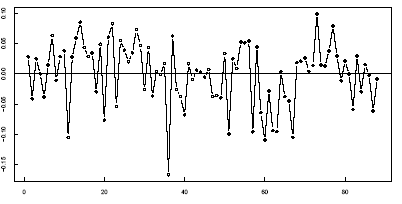
\includegraphics[scale=1.1]{Group1_U.png}
  \end{tabular}
\end{tabular}

%%%%%%%%%%%%%%%%%%%%%%%%%%%%%%%%%%%%%%%%%%%%%%%%%%%%%%%%%%
\newpage
\chead{\large {\emphase{Group 1} : the two profiles with these
changes}} \foilhead[-.5in]{}

\vspace{-.5cm}

\noindent Legend: red$=$without $U$ and black$=$ with $U$.



\begin{figure}
\begin{center}
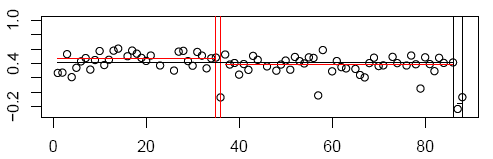
\includegraphics[scale=1]{Exemple_profile6_groupe1.png}
\end{center}
\end{figure}

\begin{figure}
\begin{center}
\includegraphics[scale=1]{Exemple_profile7_groupe1.png}
\end{center}
\end{figure}


%%%%%%%%%%%%%%%%%%%%%%%%%%%%%%%%%%%%%%%%%%%%%%%%%%%%%%%%%%
\newpage
\chead{\large { \emphase{Group 3} (results similar to groups 2 and
4) }} \foilhead[-.5in]{}

\vspace{-0.5 cm}

\begin{tabular}{c}
  \emphase{Position of the breakpoints without (red) and with (black) the random effect}\\
  \begin{tabular}{c}
  \includegraphics[scale=1.1]{Group3_rupt.png}
  \end{tabular}\\
   \emphase{Estimation of the random effect }  \\
  \begin{tabular}{c}
  \includegraphics[scale=1.1]{Group3_U.png}
  \end{tabular}
\end{tabular}


%%%%%%%%%%%%%%%%%%%%%%%%%%%%%%%%%%%%%%%%%%%%%%%%%%%%%%%%%%
\newpage
\chead{\large {\emphase{Group 3} : two profiles with these changes}}
\foilhead[-.5in]{}

\vspace{-.5cm}

\noindent Legend: red$=$without $U$ and black$=$ with $U$.




\begin{figure}
\begin{center}
\includegraphics[scale=1]{Exemple_profiles7_24_groupe3_bis.png}
\end{center}
\end{figure}

%%%%%%%%%%%%%%%%%%%%%%%%%%%%%%%%%%%%%%%%%%%%%%%%%%%%%%%%%%
\newpage
\chead{\large {Results}} \foilhead[-.5in]{}

\paragraph{Estimated variances.}
\begin{equation*}
(\widehat{\sigma}_g^2)_g=(0.0031, 0.0027 ,0.0036 ,0.0033)
\end{equation*}
$\rightarrow$ The estimated variances are similar. \\ \\

\paragraph{Random effect.}
\begin{description}
\item[$\Rightarrow$] could help to detect particular points, as
\begin{itemize}
\item
bad spot quality,
\item annotation error of the coordonnates of the
considered DNA sequence in the genome
\item or frequently deleted
position.
\end{itemize}
\end{description}

%%%%%%%%%%%%%%%%%%%%%%%%%%%%%%%%%%%%%%%%%%%%%%%%%%%%%%%%%%
%%%%%%%%%%%%%%%%%%%%%%%%%%%%%%%%%%%%%%%%%%%%%%%%%%%%%%%%%%
\newpage
\chead{\large {Perspectives}} \foilhead[-.5in]{}


\paragraph{Other application fields}
\begin{itemize}
\item Climatic data. Breakpoint detection of the evolution of the
temperature of several cities in France.
\item Botanic data. Growth phase detection of trees. \\ \\ \\
\end{itemize}
\paragraph{Develop a segmentation/clustering model} to provide biological status of the detected segments
(normal/deleted/amplified).\\

%\noindent Proposition of post doctoral position of 18 months.\\
%-Presentation of the subject:
%{\footnotesize \texttt{$http://www.inapg.fr/ens\_rech/maths/$}}\\
%-Contact: robin@inapg.inra.fr


%%%%%%%%%%%%%%%%%%%%%%%%%%%%%%%%%%%%%%%%%%%%%%%%%%%%%%%%%%
%%%%%%%%%%%%%%%%%%%%%%%%%%%%%%%%%%
% Dernier transparent
\newpage
\chead{\large {}} \foilhead[-.5in]{}


\vspace{5.5cm}

\begin{center}
\Large{Thanks for your attention}
\end{center}




\end{document}
